\documentclass[conference]{../cls/IEEEtran}

\usepackage{graphicx}

\begin{document}

\title{Early Estimation of Multi-Objective Traffic Behavior}

\author{
	\IEEEauthorblockN{Dominik Ascher}
	\IEEEauthorblockA{
		Chair IV: Software \& Systems Engineering\\
		Technische Universit\"at M\"unchen\\
		Boltzmannstr.\ 3, 85748 Garching, Germany\\
		Email: ds.ascher@gmail.com
	}
	\and
	\IEEEauthorblockN{Georg Hackenberg}
	\IEEEauthorblockA{
		Chair IV: Software \& Systems Engineering\\
		Technische Universit\"at M\"unchen\\
		Boltzmannstr.\ 3, 85748 Garching, Germany\\
		Email: hackenbe@in.tum.de
	}
}

\maketitle

\begin{abstract}
Intelligent Transportation Systems (ITS) have come a long way targeting recent problems of increasing emissions and growing vehicle numbers. Current approaches address a variety of objectives including congestion management, collision avoidance, energy-efficiency and emission reduction. However, respective solutions typically are designed for and tailored to a fixed subset of objectives. Consequently, the effects of changing objectives and priorities cannot be assessed easily. To overcome this situation we present a lightweight approach to estimating traffic behavior early in the systems engineering process using discrete-time and continuous-state system models. We demonstrate the feasibility of the framework using a basic traffic scenario before closing with a first conlusion and outlook.
\end{abstract}

\begin{IEEEkeywords}
Feasibility study, intelligent transportation systems.
\end{IEEEkeywords}

\section{Motivation}
\label{sec:motivation}

In recent decades, efforts to engineer ITS have come a long way, targeting contemporary and future problems of increasing emissions and growing vehicle numbers. Among the approaches two main directions can be distinguished: (1) Urban Traffic Control (UTC) focusing on multiple traffic participants and their interaction~\cite{Chen2010,Dresner2008} and (2) Eco-Routing focusing on a single traffic participant and his route~\cite{Ericsson2006,Boriboonsomsin2012}. In particular, UTC typically targets congestion management and collision avoidance~\cite{Chen2010}. Technically, the approaches rely on agent based techniques to describe human driving behavior with respect to traffic supervision and control~\cite{Chen2010}. More advanced approaches even consider fully autonomous vehicles thereby proposing an alternative to human-oriented traffic supervision and control~\cite{Dresner2008}. In contrast, Eco-Routing typically targets energy-efficiency and emission reduction~\cite{Ericsson2006}. Technically, the approaches rely on optimization techniques to describe route variables, constraints and objectives~\cite{Ericsson2006}. As frequent use of energy-efficient routes might cause congestion, advanced approaches finally incorporate historical and real-time traffic information thereby taking first steps towards bridging the gab between Eco-Routing and UTC~\cite{Boriboonsomsin2012}. Common among all previous approaches are objectives like congestion management, collision avoidance, energy-efficiency and emission reduction.

However, while the presented approaches offer tailored solutions for a fixed set
of objectives, they are not designed to estimate the effect of changing objectives and priorities. In particular, it is important to estimate this effect in early phases of systems engineering (such as requirements discovery or feasibility study) to uncover potential opportunities and threats~\cite{Whitten2005}. To overcome this situation in the following we present a lightweight model-based approach.

\section{A Lightweight Model-Based Approach}
\label{sec:approach}

An overview of our model-based approach to traffic behavior estimation is shown in Figure~\ref{fig:framework}. Technically, we base our work on emergent property estimation techniques described in~\cite{Hackenberg2012}. Consequently, we use a discrete-time and continuous-state system model. We rely on discrete-time models to reduce the reachable state space during behavior estimation. However, we work with continuous-state models because quantities like velocity or distance can be described more intuitively. Further, we employ a generic model architecture separating between context, constraint, objective, software and equivalence model. The non-deterministic software model describes the optimizable control behavior (not the control logic), while the context model describes the controlled physical state. Based on the physical state the constraint and objective models define the operational limits and costs. Finally, the equivalence model describes how the physical states can be clustered during optimization. For control behavior estimation the framework finally integrates stochastic approximation techniques~\cite{Pereira1991} to achieve robustness against arbitrary cost functions/constraints.
\begin{figure}[h]
	\centering
	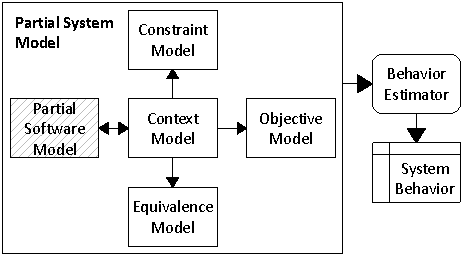
\includegraphics{../gfx/framework.pdf}
	\caption{Overview of the model-based approach to traffic behavior estimation.}
	\label{fig:framework}
\end{figure}

\section{Its Application to Traffic Systems}

In the following we apply the approach to a basic traffic scenario including
various participants as well as common time and energy objectives.
First, we describe the model before
presenting behavior estimates for different objective weights.

\subsubsection{Model}

To reduce the physical state space for behavior estimation, in our model the
traffic infrastructure is represented as a directed graph consisting of nodes and edges. Nodes constitute reference points in the environment such as junctions and are defined by their absolute position, i.e.
latitude, longitude and elevation. Edges represent road segments and are defined
by source and target node as well as assigned number of
lanes.
Finally, for demonstration we use a time resolution of 60 seconds, but other
resolutions are supported as well.

The \textit{context model} \ldots Vehicles
context component's behavior is defined by relative position on the edge, vehicle energy
consumption and state of charge. Within a time interval, energy consumption
is estimated via the current edge's altitude difference and selected
vehicle speed in the time interval. Vehicle speed relates quadratically to
current energy consumption. 
The \textit{constraint model} \ldots
Firstly, for collision avoidance, within the constraint
component of the traffic system, a collision constraint tests for every
edge within the traffic system, whether the relative positions of inhabiting
vehicles on the edge overlap. In this case, it determines, based on the number of traffic
lanes assigned to the edge, whether there are free lanes available on the
current position.
The \textit{objective model} \ldots
Secondly, in the objective component of vehicles, two main
objectives are defined: energy-efficiency and shortest travelling time.
Shortest travelling time is realized as
an objective function by minimization of indicated travelling time, while the
objective function for energy-efficiency is formulated by minimization of vehicle
energy consumption in relation to maximum possible energy consumption.
For adjusting priorities of objectives and traffic
behavior, the cost functions (objectives) are attributed with adjustable
weights.
The \textit{software model} \ldots
In vehicles, the non-deterministic control spectrum of the control
component is essentially defined by speed and edge selection.
Edge selection is based on the available choices on the current position of the observed
vehicle, while speed selection is made based on a continuous value range and
represents the traversed distance by the vehicle per time interval.
The \textit{equivalence model} \ldots 
Furthermore, in the equivalence component, the
vehicles state of charge is defined as an equivalence for clustering during state-space exploration.

\subsubsection{Analysis}

For evaluating our approach, we develop a basic traffic scenario
including multiple vehicles within the traffic infrastructure: Each vehicle has
the same origin and the same destination. There are two different
routes for vehicles to drive from origin to destination. The first route
represents a longer, but flat route, while the second route describes a shorter,
but undulating route.
To demonstrate behavior estimation, we analyze two weight configurations of the
energy and time objectives.
Configuration A favors lower energy consumption, while
configuration B favors shorter travel time.

According results for the resulting traffic behavior of the two configurations
are depicted in Figure 2, showing resulting route selection and aggregated
energy consumption for vehicles over time. Configuration A shows, for the
majority of traffic, affinity to more energy-efficient (flat) route selection
and, compared to configuration B, less energy consumption. Configuration B
exerts vehicle driving behavior towards shortest time through increased energy
consumption, but less elapsed time. Congestion within the
traffic system limits the possibilities for according route selection and
energy consumption in regard to the respectively selected weighting of
objectives. Therefore, simulation results represent a
possible trade-off between favored objectives and congestion emergence.

\begin{figure}[t!]
	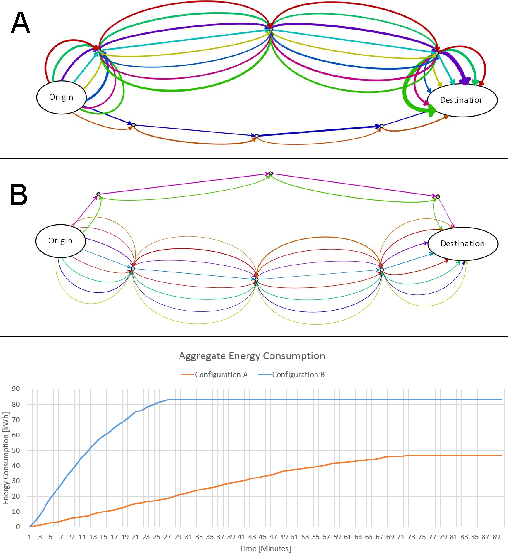
\includegraphics[width=\columnwidth]{../gfx/results.pdf}
	\caption{Comparison of routes (top) and aggregate energy consumption
	(bottom) for weight preference  on (A) energy-efficient and (B) time.}
	\label{figure:results}
\end{figure}


\section{Conclusion and Outlook}

The preliminary results are encouraging with respect to the feasibility of the model-based approach for multi-objective behavior estimation in the domain of traffic systems.
Currently, we are working on a detailed description of the model, a larger-scale demonstrator and the inclusion of multi-model travelling facilities such as bycicles, trains or airplains.

\bibliographystyle{../bst/IEEEtran}
\bibliography{ICCVE-2014}

\end{document}
